%!TEX root = ../dissertation.tex

\chapter{Environment Overview}
\label{sec:network_overview}
There are many applicability domains and different methods for creating \gls{IoT} networks.
Some provide direct connectivity of nodes to the Internet while others provide a common gateway for interfacing with external networks. This main difference has profound implications on the type of devices and protocols used for communication. In the following paragraphs a short overview of these two types of architectures is presented.

\section{Large Area Networks}

\begin{figure}[h]
  \centering
  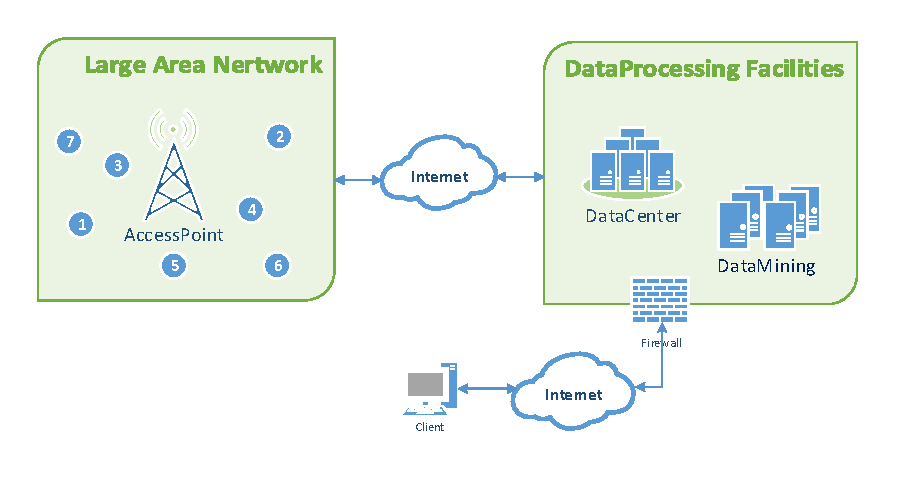
\includegraphics[width=0.85\linewidth]{figures/Network_Overview_Sparse.pdf}
  \caption{IoT Large Area Network Overview.}
  \label{fig:net_overview_large}
\end{figure}

In this type of architectures, the network nodes transmit sensing information to global access points without requiring inter-devices communication. The access point can range from routers, to GSM towers of even satellites. The outgoing messages and then transmitted through the Internet to external data processing facilities, where large amounts of data from many sources are converted into useful information on demand. This information can then be access by the users from outside the site, also through the Internet.
This type of deployments could be used, for example, in Smart Cities, where there is the need to cover a large area with sensors. A typical scenario would be to collect information on the city garbage bins to make dynamic collection routes based on the status of the recipient.
  
\section{Personal Area Networks}

\begin{figure}[h]
  \centering
  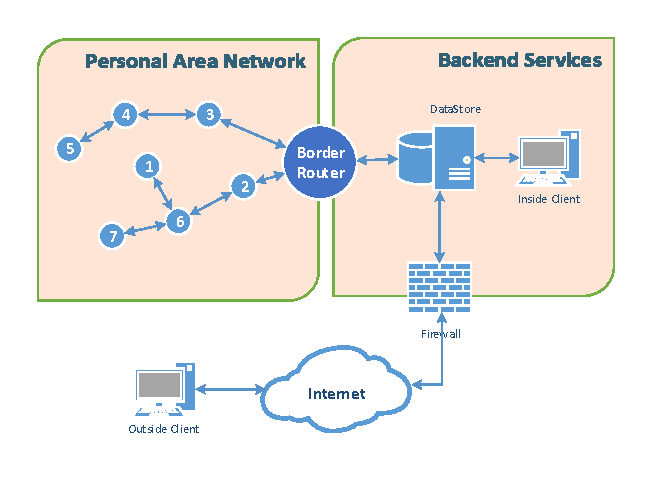
\includegraphics[width=0.8\linewidth]{figures/Network_Overview.pdf}
  \caption{IoT Personal Area Network Overview.}
  \label{fig:net_overview_small}
\end{figure}

In this type of architectures, the sensing or actuating nodes belong to a very constrained network with specific protocols and header compression mechanisms, requiring an interface device -- the border router -- in order to communicate with external networks.
After reaching the external network, incoming messages are processed to convert sensor data into useful information which is then stored or used to trigger events. 
This information can then be accessed by users either on the same network or by making requests through the Internet. 
This type of deployment could be used, for example, in a home intrusion system where the network nodes would create a sensor network that propagates events in the case of an intrusion and the additional infrastructure would be in charge of receiving these events and notifying the police authorities.\\
 
Given the power-aware focus of our work, the personal area networks architecture allows a greater resource consumptions reduction because of its communication model. Furthermore, since the back-end facilities are usually present in the same site as the network, there is the possibility of adding external components to allow the inclusion of our solution. With these two aspects in mind, in our work we focus on the scenarios where network nodes are not directly connected to the Internet and require additional network components for proper communication.